\chapter{Projections}

A projection describes the relationship of one vector to another in terms of direction and orthogonality. Given two vectors, $\mathbf{u}$ and $\mathbf{v}$, the projection of $\mathbf{u}$ onto $\mathbf{v}$ separates $\mathbf{u}$ into two components. The first component signifies how much $\mathbf{u}$ lies in the direction of $\mathbf{v}$. The second signifies the component of $\mathbf{u}$ that is orthogonal (perpendicular) to $\mathbf{v}$. \index{projection} The figure depicts a projection. The perpendicular line dropped from the end of $\mathbf{u}$ is the orthogonal component. The portion of $\mathbf{u}$ that lies in the direction of $\mathbf{v}$ is the blue segment. 


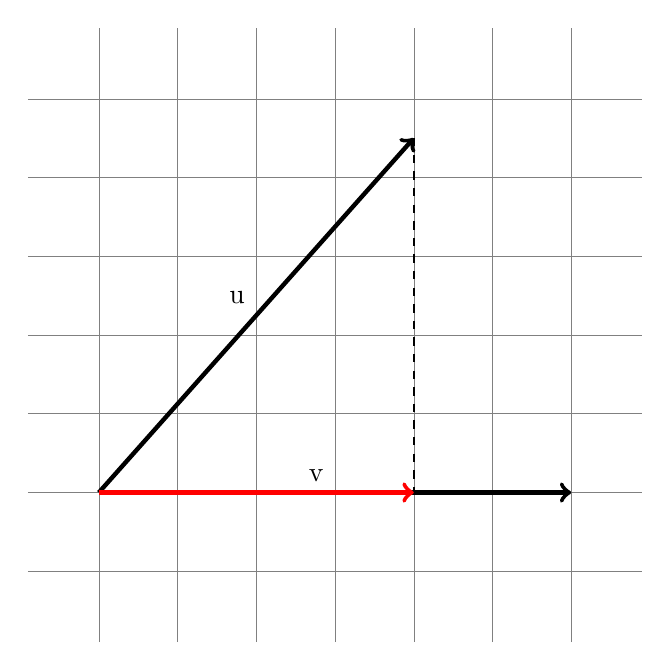
\begin{tikzpicture}
%\draw[gray,->] (0,0)-- (9.0,0) node[anchor=north west] {x axis};
%\draw[gray,->] (0,0)-- (0, 9.0) node[anchor=south east] {y axis};

\draw[step=1cm, gray, very thin](-1.9, -1.9) grid (5.9,5.9);
\draw[black, ultra thick, ->] (-1,0) -- (3,4.5) node[midway,above left] {u};
\draw[black, ultra thick, ->] (-1,0) -- (5,0) node[midway,above left] {v};
\draw[black, thick, dashed] (3,4.5) -- (3,0);
\draw[red, ultra thick, ->] (-1,0) -- (3,0);

\end{tikzpicture}


You can also think of a projection as the shadow cast by one vector onto each other by an overhead light.

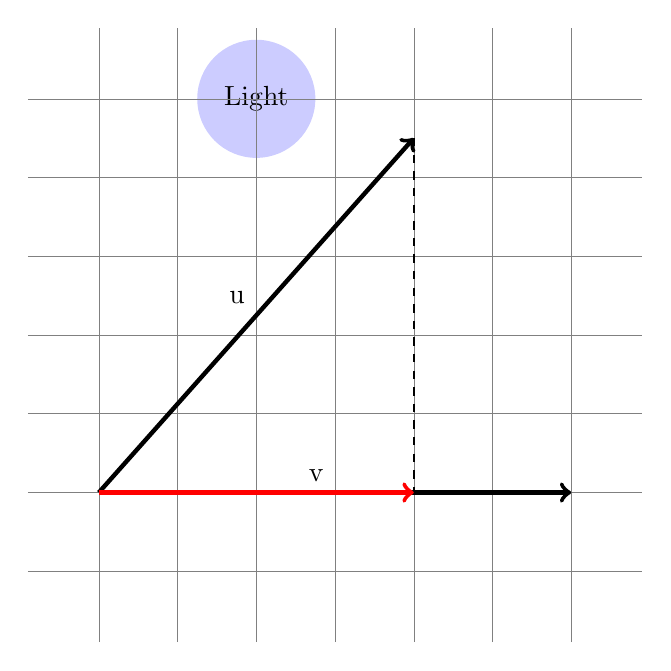
\begin{tikzpicture}[fatnode/.style={circle, fill=blue!20, minimum size=15mm}]

\node[fatnode] (A) at (1, 5) {Light};
\draw[step=1cm, gray, very thin](-1.9, -1.9) grid (5.9,5.9);

\draw[black, ultra thick, ->] (-1,0) -- (3,4.5) node[midway,above left] {u};
\draw[black, ultra thick, ->] (-1,0) -- (5,0) node[midway,above left] {v};
\draw[black, thick, dashed] (3,4.5) -- (3,0);
\draw[red, ultra thick, ->] (-1,0) -- (3,0);

\end{tikzpicture}


The projected vector can be in any direction. The length of the projected vector can extend beyond the vector on which it is projecting.

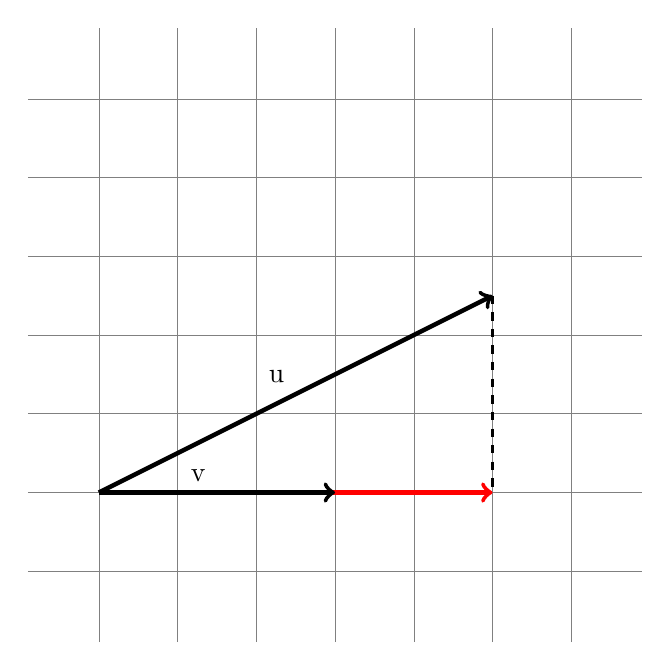
\begin{tikzpicture}  
\draw[step=1cm, gray, very thin](-1.9, -1.9) grid (5.9,5.9);
\draw[black, ultra thick, ->] (-1,0) -- (4,2.5)node[midway,above left] {u};
\draw[red, ultra thick, ->] (-1,0) -- (4,0);
\draw[black, ultra thick, ->] (-1,0) -- (2,0)node[midway,above left] {v};
\draw[black, thick, dashed] (4,2.5) -- (4,0);
\end{tikzpicture}

Projections are useful in many fields. These are a few examples, but there are numerous other applications in science, math, engineering, and finance.

\begin{itemize}
\item Investors evaluate risk and return of a portfolio by projecting an asset’s return onto a reference portfolio.
\item Astronomers analyze the motion of stellar objects by projecting the object’s true motion onto the plane of the sky.
\item Robotics engineers use projections to prevent robots from running into obstacles by projecting the robot’s position onto the optimal path.
\end{itemize}

As you work your way through this course, you'll have a chance to apply the calculations you learn in this chapter to a variety of problems. Specifically, the next chapter shows how to transform a set of linearly independent vectors into a set of orthogonal ones. Projections are essential to that transformation. 

To calculate the projection of 
$\mathbf{v}$ onto $\mathbf{u}$,use this formula:

$$\mathbf{proj}_\mathbf{v}(\mathbf{u}) = \frac{u\cdot v}{\parallel{v}\parallel ^2}v$$

Note that the denominator is is the magnitude squared of vector v.
$$(\sqrt{a_1^2 + a_2^2 + ... + a_n^2} )^2$$
You learned previously that this is the same as the dot product of a vector with itself.
$${v\cdot v}$$
In the examples that follow, we'll simplify to the dot product notation.

Let's look at a specific example:

$$u = (1,4,6)$$ 
$$v = (-2,6,2)$$ 

$$\mathbf{proj}_\mathbf{v}(\mathbf{u}) = \frac{u\cdot v}{\parallel {v}\parallel ^2}v$$
$$\mathbf{proj}_\mathbf{v}(\mathbf{u}) = \frac{(1,4,6)\cdot(-2,6,2)}{ (-2,6,2)\cdot (-2,6,2)}(-2,6,2)$$
$$\mathbf{proj}_\mathbf{v}(\mathbf{u}) = (\frac{34}{44}(-2,6,2)$$
$$\mathbf{proj}_\mathbf{v}(\mathbf{u}) = (-1.545, 4.64, 1.545)$$

\begin{Exercise}[title={Projections}, label=projections]
	Find the projection of $\mathbf{a}$ on $\mathbf{b}$ where:
	$$a = (1,3)$$
	$$b = (-4,6)$$
\end{Exercise}
\begin{Answer}[ref=project_vector]
	Compute dot product of $\mathbf{a}$ and $\mathbf{b}$:
	$$1*-4 + 3*6 = -4 +18 = 14$$
	Compute the dot product of $\mathbf{b}$ and $\mathbf{b}$
	$$16 + 36 = 52 $$
	$$14/52 * (-4,6) = (-1.076 , 1.61)$$
\end{Answer}
 
\section{Projections in Python}

Create a file called \filename{vectors\_projections.py} and enter this code:
\begin{Verbatim}
import numpy as np
  
a = np.array([1, 4, 6])   # vector a
b = np.array([-2, 6, 2])   # vector b
  
# Use np.dot() to calculate the dot product
projection_a_on_b = (np.dot(a, b)/np.dot(b, b))*b
  
print("The projection of vector a on vector b is:", projection_a_on_b)
\end{Verbatim}
 
\section{Where to Learn More}

Watch this Introduction to Projections from Khan Academy 
\url{https://rb.gy/yf0i3}

